La agricultura enfrenta desafíos crecientes en la optimización de la
productividad y la eficiencia, especialmente en regiones con condiciones
climáticas adversas y variables. Los sistemas de cultivo tradicionales suelen
ser ineficientes en la gestión de recursos esenciales como agua, nutrientes y
energía, en gran parte debido a la falta de monitoreo en tiempo real, lo que
afecta negativamente tanto la calidad como el rendimiento de los cultivos.
Además, los agricultores se enfrentan a altos costos operativos y a un impacto
negativo en la sostenibilidad ambiental debido a prácticas no optimizadas. Ante
estas dificultades, los cultivos hidropónicos han surgido como una solución
mejorada, permitiendo una utilización más eficiente de los recursos.

El presente trabajo se desarrollará en los invernaderos de la unidad hidropónica de la Facultad de 
Ciencias Forestales (FCF) de la Universidad Nacional de Misiones (UNaM).
En la actualidad, estos invernaderos utilizan un sistema de control con temporizadores que 
operan sin tener en cuenta las variables ambientales, lo que implica que la intervención 
humana debe ser continua y las mediciones de temperatura, potencial de Hidrógeno (pH) y
conductividad eléctrica (CE) de la solución nutritiva se realiza de forma manual. Esta falta 
de monitoreo en tiempo real afecta negativamente la calidad y el rendimiento de los cultivos. 
Además, esto conlleva a altos costos operativos y un impacto negativo en la sostenibilidad  
ambiental debido a prácticas no optimizadas.

La propuesta, como puede observarse en la figura \ref{fig:diagBloques}, consiste
en desarrollar un conjunto de sensores y actuadores basados en el microcontrolador ESP32. Estos dispositivos 
se conectan a un servidor IoT en la nube a través de Wi-Fi y envían los datos mediante el protocolo MQTT 
(\textit{Message Queue Telemetry Transport}). Esta configuración permitirá monitorear y gestionar el sistema 
de manera remota desde una aplicación web del tipo SPA (\textit{Single Page Application}).


\begin{figure}[htpb]
	\centering
	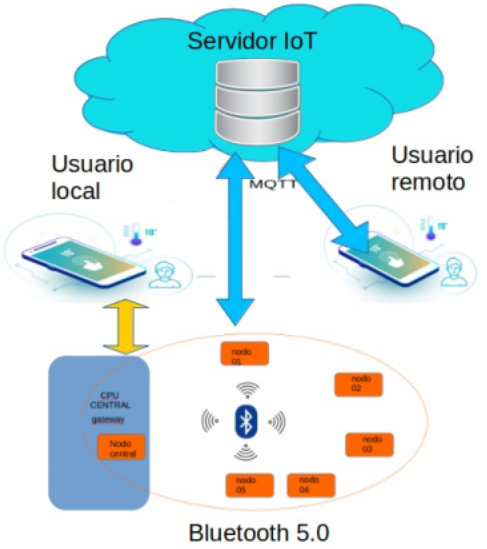
\includegraphics[width=.85\textwidth]{./Figuras/figura1.png}
	\caption{Diagrama en bloques del sistema.}
	\label{fig:diagBloques}
\end{figure}

Esta solución proporcionará un control más preciso sobre los cultivos, mejorará la eficiencia en la gestión del 
clima y optimizará el uso de los recursos. Esto se traducirá en una mayor productividad, una reducción de los  
costos operativos y una gestión más sostenible de los cultivos.